\documentclass[11pt,
  english,
  a4paper,
]{article}
\usepackage{sa4ss}
\usepackage{amsmath,amssymb,array}
\usepackage{booktabs}

% From tagged-template.latex
\usepackage{lmodern}
\usepackage{ifxetex,ifluatex}
\ifnum 0\ifxetex 1\fi\ifluatex 1\fi=0 % if pdftex
  \usepackage[T1]{fontenc}
  \usepackage[utf8]{inputenc}
  \usepackage{textcomp} % provide euro and other symbols
\else % if luatex or xetex
  \usepackage{unicode-math}
  \defaultfontfeatures{Scale=MatchLowercase}
  \defaultfontfeatures[\rmfamily]{Ligatures=TeX,Scale=1}
\fi

% Use upquote if available, for straight quotes in verbatim environments
\IfFileExists{upquote.sty}{\usepackage{upquote}}{}
\IfFileExists{microtype.sty}{% use microtype if available
  \usepackage[]{microtype}
  \UseMicrotypeSet[protrusion]{basicmath} % disable protrusion for tt fonts
}{}
\makeatletter
\@ifundefined{KOMAClassName}{% if non-KOMA class
  \IfFileExists{parskip.sty}{%
    \usepackage{parskip}
  }{% else
    \setlength{\parindent}{0pt}
    \setlength{\parskip}{6pt plus 2pt minus 1pt}}
}{% if KOMA class
  \KOMAoptions{parskip=half}}
\makeatother
\usepackage{xcolor}
\IfFileExists{xurl.sty}{\usepackage{xurl}}{} % add URL line breaks if available
\hypersetup{
  pdftitle={Status of copper rockfish (Sebastes caurinus) along the Washigton US West coast in 2020},
  pdflang={en},
  hidelinks,
  pdfcreator={LaTeX via pandoc}}
\urlstyle{same} % disable monospaced font for URLs
\usepackage{longtable}
% Correct order of tables after \paragraph or \subparagraph
\usepackage{etoolbox}
\makeatletter
\patchcmd\longtable{\par}{\if@noskipsec\mbox{}\fi\par}{}{}
\makeatother
% Allow footnotes in longtable head/foot
\IfFileExists{footnotehyper.sty}{\usepackage{footnotehyper}}{\usepackage{footnote}}
\makesavenoteenv{longtable}
\usepackage{graphicx}
\makeatletter
\def\maxwidth{\ifdim\Gin@nat@width>\linewidth\linewidth\else\Gin@nat@width\fi}
\def\maxheight{\ifdim\Gin@nat@height>\textheight\textheight\else\Gin@nat@height\fi}
\makeatother
% Scale images if necessary, so that they will not overflow the page
% margins by default, and it is still possible to overwrite the defaults
% using explicit options in \includegraphics[width, height, ...]{}
\setkeys{Gin}{width=\maxwidth,height=\maxheight,keepaspectratio}
% Set default figure placement to htbp
\makeatletter
\def\fps@figure{htbp}
\makeatother
\setlength{\emergencystretch}{3em} % prevent overfull lines
\providecommand{\tightlist}{%
  \setlength{\itemsep}{0pt}\setlength{\parskip}{0pt}}
\setcounter{secnumdepth}{5}
\ifxetex
  % Load polyglossia as late as possible: uses bidi with RTL langages (e.g. Hebrew, Arabic)
  \usepackage{polyglossia}
  \setmainlanguage[]{english}
\else
  \usepackage[shorthands=off,main=english]{babel}
\fi

\providecommand{\tightlist}{%
  \setlength{\itemsep}{0pt}\setlength{\parskip}{0pt}}


\date{}
\newcommand{\trTitle}{Status of copper rockfish (\emph{Sebastes caurinus}) along the Washigton US West coast in 2020}
\newcommand{\trYear}{2020}
\newcommand{\trMonth}{December}
\newcommand{\trAuthsLong}{truetruetruetruetrue}
\newcommand{\trAuthsBack}{Wetzel, C.R., B.J. Langseth, J.M. Cope, T. Tsou, K.E. Hinton}
\newcommand{\trCitation}{
\begin{hangparas}{1em}{1}
\trAuthsBack{}. \trYear{}. \trTitle{}. Pacific Fisheries Management Council, Portland, Oregon. \pageref{LastPage}{}\,p.
\end{hangparas}}

\AtBeginDocument{\tagstructbegin{tag=Document}}
\AtEndDocument{\tagstructend}
\pretocmd{\maketitle}{\tagstructbegin{tag=H1}\tagmcbegin{tag=H1}}{}{}
\apptocmd{\maketitle}{\tagmcend\tagstructend}{}{}

\begin{document}

%%%%% Frontmatter %%%%%

% Footnote symbols in front matter
\renewcommand*{\thefootnote}{\fnsymbol{footnote}}

\small
\thispagestyle{empty}
\pagenumbering{roman}
\noindent
\begin{center}
\title{Status of copper rockfish (\emph{Sebastes caurinus}) along the Washigton US West coast in 2020}
% \textnormal{\MakeTextUppercase{\trTitle{}}}
\vspace{1.5cm}
{\Large\textbf\newline{Status of copper rockfish (\emph{Sebastes caurinus}) along the Washigton US West coast in 2020}}
\vfill
by\\
Chantel R. Wetzel\textsuperscript{1}\\
Brian J. Langseth\textsuperscript{1}\\
Jason M. Cope\textsuperscript{1}\\
Tien-Shui Tsou\textsuperscript{2}\\
Kristen E. Hinton\textsuperscript{2}\vfill
\textsuperscript{1}Northwest Fisheries Science Center, U.S. Department of Commerce, National Oceanic and Atmospheric Administration, National Marine Fisheries Service, 2725 Montlake Boulevard East, Seattle, Washington 98112\\
\textsuperscript{2}Washington Department of Fish and Wildlife, 600 Capital Way North, Olympia, Washington 98501\vfill
\trMonth{} \trYear{}
\end{center}
\clearpage

% Fourth page: Colophon
\thispagestyle{empty}
\vspace*{\fill}
\begin{center}
\copyright{} Pacific Fisheries Management Council, \trYear{}\\
\end{center}
\par
\bigskip
\noindent
Correct citation for this publication:
\bigskip
\par
\trCitation{}
\clearpage

% Add TOC to pdf bookmarks (clickable pdf)
\pdfbookmark[1]{\contentsname}{toc}

% Table of contents page, lists of figures and tables
\tableofcontents\clearpage
\listoffigures \listoftables \clearpage
\label{TRlastRoman}
\clearpage

% Table of contents
\newpage
\thispagestyle{empty} % to remove page number

% Settings for the main document
\pagenumbering{arabic}  % Regular page numbers
\pagestyle{plain}  % No page number on first page of main document, use 'empty'
\renewcommand*{\thefootnote}{\arabic{footnote}}  % Back to numeric footnotes
\setcounter{footnote}{0}  % And start at 1
\renewcommand{\headrulewidth}{0.5pt}
\renewcommand{\footrulewidth}{0.5pt}
%\pagestyle{fancy}\fancyhead[c]{Draft: Do not cite or circulate}

\newcommand{\lt}{\ensuremath <}
\newcommand{\gt}{\ensuremath >}

%Define cslreferences environment, required by pandoc 2.8
%https://github.com/rstudio/rmarkdown/issues/1649
\newlength{\cslhangindent}
\setlength{\cslhangindent}{1.5em}
\newenvironment{cslreferences}%
  {\setlength{\parindent}{0pt}%
  \everypar{\setlength{\hangindent}{\cslhangindent}}\ignorespaces}%
  {\par}

\pagebreak
\pagenumbering{roman}
\setcounter{page}{1}
\renewcommand{\thetable}{\roman{table}}
\renewcommand{\thefigure}{\roman{figure}}

\pagebreak
\setlength{\parskip}{5mm plus1mm minus1mm}
\pagenumbering{arabic}
\setcounter{page}{1}
\renewcommand{\thefigure}{\arabic{figure}}
\renewcommand{\thetable}{\arabic{table}}
\setcounter{table}{0}
\setcounter{figure}{0}

\tagstructbegin{tag=H1}\tagmcbegin{tag=H1}

\hypertarget{introduction}{%
\section{Introduction}\label{introduction}}

\leavevmode\tagmcend\tagstructend

\tagstructbegin{tag=H2}\tagmcbegin{tag=H2}

\hypertarget{basic-information}{%
\subsection{Basic Information}\label{basic-information}}

\leavevmode\tagmcend\tagstructend

\tagstructbegin{tag=P}\tagmcbegin{tag=P}

This assessment reports the status of copper rockfish (\emph{Sebastes caurinus}) off the US West coast using data through 2020. Copper rockfish is a medium- to large-sized nearshore rockfish found from Mexico to Alaska. The core range is comparatively large, from northern Baja Mexico to the Gulf of Alaska, as well as in Puget Sound. They occur mostly on low relief or sand-rock interfaces. Copper rockfish have historically been a part of both commercial (mainly in the live-fish fishery) and recreational fisheries throughout its range.

\leavevmode\tagmcend\tagstructend\par

\tagstructbegin{tag=H2}\tagmcbegin{tag=H2}

\hypertarget{life-history}{%
\subsection{Life History}\label{life-history}}

\leavevmode\tagmcend\tagstructend

\tagstructbegin{tag=P}\tagmcbegin{tag=P}

Genetic work has revealed significant differences between Puget Sound and coastal stocks, but not among the coastal stocks (XXX Buonaccorsi et al.~2002). copper rockfish live at least 50 years (XX add reference XX) and have the highest vulnerability (V = 2.27) of any West Coast groundfish (XX add reference XX).

\leavevmode\tagmcend\tagstructend\par

\tagstructbegin{tag=H2}\tagmcbegin{tag=H2}

\hypertarget{ecosystem-considerations}{%
\subsection{Ecosystem Considerations}\label{ecosystem-considerations}}

\leavevmode\tagmcend\tagstructend

\tagstructbegin{tag=P}\tagmcbegin{tag=P}

Replace text.

\leavevmode\tagmcend\tagstructend\par

\tagstructbegin{tag=H2}\tagmcbegin{tag=H2}

\hypertarget{historical-and-current-fishery-information}{%
\subsection{Historical and Current Fishery Information}\label{historical-and-current-fishery-information}}

\leavevmode\tagmcend\tagstructend

\tagstructbegin{tag=P}\tagmcbegin{tag=P}

Replace text.

\leavevmode\tagmcend\tagstructend\par

\tagstructbegin{tag=H2}\tagmcbegin{tag=H2}

\hypertarget{summary-of-management-history-and-performance}{%
\subsection{Summary of Management History and Performance}\label{summary-of-management-history-and-performance}}

\leavevmode\tagmcend\tagstructend

\tagstructbegin{tag=P}\tagmcbegin{tag=P}

Replace text.

\leavevmode\tagmcend\tagstructend\par

\tagstructbegin{tag=H2}\tagmcbegin{tag=H2}

\hypertarget{foreign-fisheries}{%
\subsection{Foreign Fisheries}\label{foreign-fisheries}}

\leavevmode\tagmcend\tagstructend

\tagstructbegin{tag=P}\tagmcbegin{tag=P}

Replace text.

\leavevmode\tagmcend\tagstructend\par

\tagstructbegin{tag=H1}\tagmcbegin{tag=H1}

\hypertarget{data}{%
\section{Data}\label{data}}

\leavevmode\tagmcend\tagstructend

\tagstructbegin{tag=P}\tagmcbegin{tag=P}

A description of each data source is provided below (Figure \ref{fig:data-plot}).

\leavevmode\tagmcend\tagstructend\par

\tagstructbegin{tag=H2}\tagmcbegin{tag=H2}

\hypertarget{fishery-dependent-data}{%
\subsection{Fishery-Dependent Data}\label{fishery-dependent-data}}

\leavevmode\tagmcend\tagstructend

\tagstructbegin{tag=P}\tagmcbegin{tag=P}

{\tagstructbegin{tag=Reference}\tagmcbegin{tag=Reference}(Ralston et al. 2010)\leavevmode\tagmcend\tagstructend}

\leavevmode\tagmcend\tagstructend\par

\tagstructbegin{tag=H2}\tagmcbegin{tag=H2}

\hypertarget{fishery-independent-data}{%
\subsection{Fishery-Independent Data}\label{fishery-independent-data}}

\leavevmode\tagmcend\tagstructend

\tagstructbegin{tag=P}\tagmcbegin{tag=P}

There were no fishery-independent data sources available for copper rockfish off the Washington coast to be considered for this assessment.

\leavevmode\tagmcend\tagstructend\par

\tagstructbegin{tag=H2}\tagmcbegin{tag=H2}

\hypertarget{biological-data}{%
\subsection{Biological Data}\label{biological-data}}

\leavevmode\tagmcend\tagstructend

\tagstructbegin{tag=H3}\tagmcbegin{tag=H3}

\hypertarget{natural-mortality}{%
\subsubsection{Natural Mortality}\label{natural-mortality}}

\leavevmode\tagmcend\tagstructend

\tagstructbegin{tag=P}\tagmcbegin{tag=P}

Hamel {\tagstructbegin{tag=Reference}\tagmcbegin{tag=Reference}(2015)\leavevmode\tagmcend\tagstructend} developed a method for combining meta-analytic approaches relating the {\tagstructbegin{tag=Formula}\tagmcbegin{tag=Formula}\(M\)\leavevmode\tagmcend\tagstructend} rate to other life-history parameters such as longevity, size, growth rate, and reproductive effort to provide a prior on {\tagstructbegin{tag=Formula}\tagmcbegin{tag=Formula}\(M\)\leavevmode\tagmcend\tagstructend}. In that same issue of \emph{ICES Journal of Marine Science}, Then et al.~{\tagstructbegin{tag=Reference}\tagmcbegin{tag=Reference}(2015)\leavevmode\tagmcend\tagstructend} provided an updated data set of estimates of {\tagstructbegin{tag=Formula}\tagmcbegin{tag=Formula}\(M\)\leavevmode\tagmcend\tagstructend} and related life history parameters across a large number of fish species from which to develop an {\tagstructbegin{tag=Formula}\tagmcbegin{tag=Formula}\(M\)\leavevmode\tagmcend\tagstructend} estimator for fish species in general. They concluded by recommending {\tagstructbegin{tag=Formula}\tagmcbegin{tag=Formula}\(M\)\leavevmode\tagmcend\tagstructend} estimates be based on maximum age alone, based on an updated Hoenig non-linear least squares estimator {\tagstructbegin{tag=Formula}\tagmcbegin{tag=Formula}\(M=4.899A^{-0.916}_{max}\)\leavevmode\tagmcend\tagstructend}. The approach of basing {\tagstructbegin{tag=Formula}\tagmcbegin{tag=Formula}\(M\)\leavevmode\tagmcend\tagstructend} priors on maximum age alone was one that was already being used for West Coast rockfish assessments. However, in fitting the alternative model forms relating {\tagstructbegin{tag=Formula}\tagmcbegin{tag=Formula}\(M\)\leavevmode\tagmcend\tagstructend} to {\tagstructbegin{tag=Formula}\tagmcbegin{tag=Formula}\(A_{\text{max}}\)\leavevmode\tagmcend\tagstructend}, Then et al.~{\tagstructbegin{tag=Reference}\tagmcbegin{tag=Reference}(2015)\leavevmode\tagmcend\tagstructend} did not consistently apply their transformation. In particular, in real space, one would expect substantial heteroscedasticity in both the observation and process error associated with the observed relationship of {\tagstructbegin{tag=Formula}\tagmcbegin{tag=Formula}\(M\)\leavevmode\tagmcend\tagstructend} to {\tagstructbegin{tag=Formula}\tagmcbegin{tag=Formula}\(A_{\text{max}}\)\leavevmode\tagmcend\tagstructend}. Therefore, it would be reasonable to fit all models under a log transformation. This was not done. Re-evaluating the data used in Then et al.~{\tagstructbegin{tag=Reference}\tagmcbegin{tag=Reference}(2015)\leavevmode\tagmcend\tagstructend} by fitting the one-parameter {\tagstructbegin{tag=Formula}\tagmcbegin{tag=Formula}\(A_{\text{max}}\)\leavevmode\tagmcend\tagstructend} model under a log-log transformation (such that the slope is forced to be -1 in the transformed space Hamel {\tagstructbegin{tag=Reference}\tagmcbegin{tag=Reference}(2015)\leavevmode\tagmcend\tagstructend}), the point estimate for {\tagstructbegin{tag=Formula}\tagmcbegin{tag=Formula}\(M\)\leavevmode\tagmcend\tagstructend} is:

\leavevmode\tagmcend\tagstructend\par

\begin{centering}

$M=\frac{5.4}{A_{\text{max}}}$

\end{centering}

\tagstructbegin{tag=P}\tagmcbegin{tag=P}

The above is also the median of the prior. The prior is defined as a lognormal distribution with mean {\tagstructbegin{tag=Formula}\tagmcbegin{tag=Formula}\(ln(5.4/A_{\text{max}})\)\leavevmode\tagmcend\tagstructend} and SE = 0.438. Using a maximum age of 50, the point estimate and median of the prior is 0.108 per year The maximum age was selected based on available age data from all West Coast data sources and literature values. The oldest aged rockfish was 51 years with two observations, off the coast of Washington and Oregon in 2019. However, age data are subject to ageing error which could impact this estimate of longevity. The selection of 50 years was based on the range of other ages available with multiple observations of fish between 44 and 51 years of age and literature examining the longevity of \texttt{spp} {\tagstructbegin{tag=Reference}\tagmcbegin{tag=Reference}(Love 1996)\leavevmode\tagmcend\tagstructend}.

\leavevmode\tagmcend\tagstructend\par

\tagstructbegin{tag=H3}\tagmcbegin{tag=H3}

\hypertarget{maturation-and-fecundity}{%
\subsubsection{Maturation and Fecundity}\label{maturation-and-fecundity}}

\leavevmode\tagmcend\tagstructend

\tagstructbegin{tag=P}\tagmcbegin{tag=P}

NEED TO UPDATE WHEN MELISSA IS DONE

\leavevmode\tagmcend\tagstructend\par

\tagstructbegin{tag=P}\tagmcbegin{tag=P}

Maturity-at-length based on the work of Hannah XXX which estimated the 50\% size-at-maturity of 34.83 cm off the coast of Oregon with maturity asymptoting to 1.0 for larger fish (Figure ADD FIGURE).

\leavevmode\tagmcend\tagstructend\par

\tagstructbegin{tag=P}\tagmcbegin{tag=P}

This assessment assumed a logistic maturity-at-length curve based on analysis of XXX fish maturity samples collected from the NWFSC WCGBT and NWFSC Hook \& Line surveys. The new maturity-at-length curve is based on the estimate of functional maturity, an approach that classifies rockfish maturity with developing oocytes as mature or immature based on the proportion of vitellogenin in the cytoplasm and the measured frequency of atretic cells (Melissa Head, personal communication, NWFSC, NOAA). The 50\% size-at-maturity was estimated at XX cm with maturity asymptoting to 1.0 for larger fish (Figure ADD FIGURE).

\leavevmode\tagmcend\tagstructend\par

\tagstructbegin{tag=P}\tagmcbegin{tag=P}

The fecundity-at-length was based on research Dick et al.~{\tagstructbegin{tag=Reference}\tagmcbegin{tag=Reference}(2017)\leavevmode\tagmcend\tagstructend}. The fecundity relationship for copper rockfish was estimated equal to 3.362e-07{\tagstructbegin{tag=Formula}\tagmcbegin{tag=Formula}\(L\)\leavevmode\tagmcend\tagstructend}\textsuperscript{3.68} in millions of eggs where {\tagstructbegin{tag=Formula}\tagmcbegin{tag=Formula}\(L\)\leavevmode\tagmcend\tagstructend} is length in cm. Fecundity-at-length is shown in Figure ADD FIGURE.

\leavevmode\tagmcend\tagstructend\par

\tagstructbegin{tag=H3}\tagmcbegin{tag=H3}

\hypertarget{sex-ratio}{%
\subsubsection{Sex Ratio}\label{sex-ratio}}

\leavevmode\tagmcend\tagstructend

\tagstructbegin{tag=P}\tagmcbegin{tag=P}

There was limited sex specific observations by length or age for all biological data sources. The sex ratio of young fish was assumed to be 1:1.

\leavevmode\tagmcend\tagstructend\par

\tagstructbegin{tag=H3}\tagmcbegin{tag=H3}

\hypertarget{length-weight-relationship}{%
\subsubsection{Length-Weight Relationship}\label{length-weight-relationship}}

\leavevmode\tagmcend\tagstructend

\tagstructbegin{tag=P}\tagmcbegin{tag=P}

The length-weight relationship for copper rockfish was estimated outside the model using all coastwide biological data available from fishery-independent data sources, where the female weight-at-length in grams was estimated at 9.56e-06{\tagstructbegin{tag=Formula}\tagmcbegin{tag=Formula}\(L\)\leavevmode\tagmcend\tagstructend}\textsuperscript{3.19} and males at 1.08e-05{\tagstructbegin{tag=Formula}\tagmcbegin{tag=Formula}\(L\)\leavevmode\tagmcend\tagstructend}\textsuperscript{3.15} where {\tagstructbegin{tag=Formula}\tagmcbegin{tag=Formula}\(L\)\leavevmode\tagmcend\tagstructend} is length in cm (Figures ADD FIGURE).

\leavevmode\tagmcend\tagstructend\par

\tagstructbegin{tag=H3}\tagmcbegin{tag=H3}

\hypertarget{growth-length-at-age}{%
\subsubsection{Growth (Length-at-Age)}\label{growth-length-at-age}}

\leavevmode\tagmcend\tagstructend

\tagstructbegin{tag=P}\tagmcbegin{tag=P}

The length-at-age was estimated for male and female copper rockfish using data collected from fishery-dependent data sources off the coast of Oregon and Washington that were collected from 1998-2019. Figure ADD FIGURE shows the lengths and ages for all years as well as predicted von Bertalanffy fits to the data. Females grow larger than males and sex-specific growth parameters were estimated at the following values:

\leavevmode\tagmcend\tagstructend\par

\begin{centering}

Females $L_{\infty}$ = 49.6 cm; $k$ = 0.152

Males $L_{\infty}$ = 47.8 cm; $k$ = 0.182

\end{centering}

\tagstructbegin{tag=P}\tagmcbegin{tag=P}

These values were fixed within the base model for male and female copper rockfish.

\leavevmode\tagmcend\tagstructend\par

\tagstructbegin{tag=H1}\tagmcbegin{tag=H1}

\hypertarget{assessment-model}{%
\section{Assessment Model}\label{assessment-model}}

\leavevmode\tagmcend\tagstructend

\tagstructbegin{tag=H2}\tagmcbegin{tag=H2}

\hypertarget{summary-of-previous-assessments-and-reviews}{%
\subsection{Summary of Previous Assessments and Reviews}\label{summary-of-previous-assessments-and-reviews}}

\leavevmode\tagmcend\tagstructend

\tagstructbegin{tag=H3}\tagmcbegin{tag=H3}

\hypertarget{history-of-modeling-approaches-not-required-for-an-update-assessment}{%
\subsubsection{History of Modeling Approaches (not required for an update assessment)}\label{history-of-modeling-approaches-not-required-for-an-update-assessment}}

\leavevmode\tagmcend\tagstructend

\tagstructbegin{tag=H3}\tagmcbegin{tag=H3}

\hypertarget{most-recent-star-panel-and-ssc-recommendations-not-required-for-an-update-assessment}{%
\subsubsection{Most Recent STAR Panel and SSC Recommendations (not required for an update assessment)}\label{most-recent-star-panel-and-ssc-recommendations-not-required-for-an-update-assessment}}

\leavevmode\tagmcend\tagstructend

\tagstructbegin{tag=H3}\tagmcbegin{tag=H3}

\hypertarget{response-to-groundfish-subcommittee-requests-not-required-in-draft}{%
\subsubsection{Response to Groundfish Subcommittee Requests (not required in draft)}\label{response-to-groundfish-subcommittee-requests-not-required-in-draft}}

\leavevmode\tagmcend\tagstructend

\tagstructbegin{tag=H2}\tagmcbegin{tag=H2}

\hypertarget{model-structure-and-assumptions}{%
\subsection{Model Structure and Assumptions}\label{model-structure-and-assumptions}}

\leavevmode\tagmcend\tagstructend

\tagstructbegin{tag=H3}\tagmcbegin{tag=H3}

\hypertarget{model-changes-from-the-last-assessment-not-required-for-an-update-assessment}{%
\subsubsection{Model Changes from the Last Assessment (not required for an update assessment)}\label{model-changes-from-the-last-assessment-not-required-for-an-update-assessment}}

\leavevmode\tagmcend\tagstructend

\tagstructbegin{tag=H3}\tagmcbegin{tag=H3}

\hypertarget{modeling-platform-and-structure}{%
\subsubsection{Modeling Platform and Structure}\label{modeling-platform-and-structure}}

\leavevmode\tagmcend\tagstructend

\tagstructbegin{tag=P}\tagmcbegin{tag=P}

General model specifications (e.g., executable version, model structure, definition of fleets and areas)

\leavevmode\tagmcend\tagstructend\par

\tagstructbegin{tag=H3}\tagmcbegin{tag=H3}

\hypertarget{model-parameters}{%
\subsubsection{Model Parameters}\label{model-parameters}}

\leavevmode\tagmcend\tagstructend

\tagstructbegin{tag=P}\tagmcbegin{tag=P}

Describe estimated vs.~fixed parameters, priors

\leavevmode\tagmcend\tagstructend\par

\tagstructbegin{tag=H3}\tagmcbegin{tag=H3}

\hypertarget{key-assumptions-and-structural-choices}{%
\subsubsection{Key Assumptions and Structural Choices}\label{key-assumptions-and-structural-choices}}

\leavevmode\tagmcend\tagstructend

\tagstructbegin{tag=H2}\tagmcbegin{tag=H2}

\hypertarget{base-model-results}{%
\subsection{Base Model Results}\label{base-model-results}}

\leavevmode\tagmcend\tagstructend

\tagstructbegin{tag=H3}\tagmcbegin{tag=H3}

\hypertarget{parameter-estimates}{%
\subsubsection{Parameter Estimates}\label{parameter-estimates}}

\leavevmode\tagmcend\tagstructend

\tagstructbegin{tag=H3}\tagmcbegin{tag=H3}

\hypertarget{fits-to-the-data}{%
\subsubsection{Fits to the Data}\label{fits-to-the-data}}

\leavevmode\tagmcend\tagstructend

\tagstructbegin{tag=H3}\tagmcbegin{tag=H3}

\hypertarget{population-trajectory}{%
\subsubsection{Population Trajectory}\label{population-trajectory}}

\leavevmode\tagmcend\tagstructend

\tagstructbegin{tag=H3}\tagmcbegin{tag=H3}

\hypertarget{reference-points}{%
\subsubsection{Reference Points}\label{reference-points}}

\leavevmode\tagmcend\tagstructend

\tagstructbegin{tag=H2}\tagmcbegin{tag=H2}

\hypertarget{model-diagnostics}{%
\subsection{Model Diagnostics}\label{model-diagnostics}}

\leavevmode\tagmcend\tagstructend

\tagstructbegin{tag=P}\tagmcbegin{tag=P}

Describe all diagnostics

\leavevmode\tagmcend\tagstructend\par

\tagstructbegin{tag=H3}\tagmcbegin{tag=H3}

\hypertarget{convergence}{%
\subsubsection{Convergence}\label{convergence}}

\leavevmode\tagmcend\tagstructend

\tagstructbegin{tag=H3}\tagmcbegin{tag=H3}

\hypertarget{sensitivity-analyses}{%
\subsubsection{Sensitivity Analyses}\label{sensitivity-analyses}}

\leavevmode\tagmcend\tagstructend

\tagstructbegin{tag=H3}\tagmcbegin{tag=H3}

\hypertarget{retrospective-analysis}{%
\subsubsection{Retrospective Analysis}\label{retrospective-analysis}}

\leavevmode\tagmcend\tagstructend

\tagstructbegin{tag=H3}\tagmcbegin{tag=H3}

\hypertarget{likelihood-profiles}{%
\subsubsection{Likelihood Profiles}\label{likelihood-profiles}}

\leavevmode\tagmcend\tagstructend

\tagstructbegin{tag=H3}\tagmcbegin{tag=H3}

\hypertarget{unresolved-problems-and-major-uncertainties}{%
\subsubsection{Unresolved Problems and Major Uncertainties}\label{unresolved-problems-and-major-uncertainties}}

\leavevmode\tagmcend\tagstructend

\tagstructbegin{tag=H1}\tagmcbegin{tag=H1}

\hypertarget{management}{%
\section{Management}\label{management}}

\leavevmode\tagmcend\tagstructend

\tagstructbegin{tag=H2}\tagmcbegin{tag=H2}

\hypertarget{reference-points-1}{%
\subsection{Reference Points}\label{reference-points-1}}

\leavevmode\tagmcend\tagstructend

\tagstructbegin{tag=H2}\tagmcbegin{tag=H2}

\hypertarget{unresolved-problems-and-major-uncertainties-1}{%
\subsection{Unresolved Problems and Major Uncertainties}\label{unresolved-problems-and-major-uncertainties-1}}

\leavevmode\tagmcend\tagstructend

\tagstructbegin{tag=H2}\tagmcbegin{tag=H2}

\hypertarget{harvest-projections-and-decision-tables}{%
\subsection{Harvest Projections and Decision Tables}\label{harvest-projections-and-decision-tables}}

\leavevmode\tagmcend\tagstructend

\tagstructbegin{tag=H2}\tagmcbegin{tag=H2}

\hypertarget{evaluation-of-scientific-uncertainty}{%
\subsection{Evaluation of Scientific Uncertainty}\label{evaluation-of-scientific-uncertainty}}

\leavevmode\tagmcend\tagstructend

\tagstructbegin{tag=H2}\tagmcbegin{tag=H2}

\hypertarget{research-and-data-needs}{%
\subsection{Research and Data Needs}\label{research-and-data-needs}}

\leavevmode\tagmcend\tagstructend

\tagstructbegin{tag=H1}\tagmcbegin{tag=H1}

\hypertarget{acknowledgments}{%
\section{Acknowledgments}\label{acknowledgments}}

\leavevmode\tagmcend\tagstructend

\tagstructbegin{tag=P}\tagmcbegin{tag=P}

Here are all the mad props!

\leavevmode\tagmcend\tagstructend\par

\tagstructbegin{tag=P}\tagmcbegin{tag=P}

Merit McCrea, Gerry Richter, Louis Zimm, Daniel Platt

\leavevmode\tagmcend\tagstructend\par

\tagstructbegin{tag=H1}\tagmcbegin{tag=H1}

\hypertarget{tables}{%
\section{Tables}\label{tables}}

\leavevmode\tagmcend\tagstructend

\begingroup\fontsize{10}{12}\selectfont
\begingroup\fontsize{10}{12}\selectfont

\begin{longtable}[t]{r>{\centering\arraybackslash}p{2cm}>{\centering\arraybackslash}p{2cm}>{\centering\arraybackslash}p{2cm}}
\caption{\label{tab:allmortality}Removals by fleet for all model years.}\\
\toprule
Year & Recreational (mt) & Commercial (mt) & Total Mortality\\
\midrule
\endfirsthead
\caption[]{\label{tab:allmortality}Removals by fleet for all model years. \textit{(continued)}}\\
\toprule
Year & Recreational (mt) & Commercial (mt) & Total Mortality\\
\midrule
\endhead

\endfoot
\bottomrule
\endlastfoot
1935 & 0.02 & 0.00 & 0.02\\
1936 & 0.05 & 0.00 & 0.05\\
1937 & 0.09 & 0.00 & 0.09\\
1938 & 0.12 & 0.00 & 0.12\\
1939 & 0.16 & 0.00 & 0.16\\
1940 & 0.19 & 0.00 & 0.19\\
1941 & 0.23 & 0.00 & 0.23\\
1942 & 0.26 & 0.00 & 0.26\\
1943 & 0.30 & 0.00 & 0.30\\
1944 & 0.33 & 0.00 & 0.33\\
1945 & 0.37 & 0.00 & 0.37\\
1946 & 0.40 & 0.00 & 0.40\\
1947 & 0.44 & 0.00 & 0.44\\
1948 & 0.47 & 0.00 & 0.47\\
1949 & 0.51 & 0.00 & 0.51\\
1950 & 0.54 & 0.00 & 0.54\\
1951 & 0.58 & 0.00 & 0.58\\
1952 & 0.61 & 0.00 & 0.61\\
1953 & 0.64 & 0.00 & 0.64\\
1954 & 0.68 & 0.00 & 0.68\\
1955 & 0.71 & 0.00 & 0.71\\
1956 & 0.75 & 0.00 & 0.75\\
1957 & 0.78 & 0.00 & 0.78\\
1958 & 0.81 & 0.00 & 0.81\\
1959 & 0.85 & 0.00 & 0.85\\
1960 & 0.88 & 0.00 & 0.88\\
1961 & 0.91 & 0.00 & 0.91\\
1962 & 0.95 & 0.00 & 0.95\\
1963 & 0.98 & 0.00 & 0.98\\
1964 & 1.01 & 0.00 & 1.01\\
1965 & 1.05 & 0.00 & 1.05\\
1966 & 1.08 & 0.00 & 1.08\\
1967 & 1.11 & 0.00 & 1.11\\
1968 & 1.14 & 0.00 & 1.14\\
1969 & 1.18 & 0.00 & 1.18\\
1970 & 1.21 & 0.00 & 1.21\\
1971 & 1.24 & 0.00 & 1.24\\
1972 & 1.27 & 0.00 & 1.27\\
1973 & 1.31 & 0.00 & 1.31\\
1974 & 1.34 & 0.00 & 1.34\\
1975 & 1.37 & 0.00 & 1.37\\
1976 & 0.99 & 0.00 & 0.99\\
1977 & 0.61 & 0.00 & 0.61\\
1978 & 1.13 & 0.00 & 1.13\\
1979 & 1.50 & 0.00 & 1.50\\
1980 & 0.88 & 0.00 & 0.88\\
1981 & 1.96 & 0.00 & 1.96\\
1982 & 2.06 & 0.00 & 2.06\\
1983 & 1.26 & 0.00 & 1.26\\
1984 & 2.00 & 0.00 & 2.00\\
1985 & 1.72 & 0.20 & 1.92\\
1986 & 2.07 & 0.19 & 2.26\\
1987 & 2.48 & 0.93 & 3.42\\
1988 & 2.31 & 0.25 & 2.56\\
1989 & 2.34 & 0.00 & 2.34\\
1990 & 2.99 & 0.03 & 3.02\\
1991 & 2.19 & 0.00 & 2.19\\
1992 & 3.55 & 0.00 & 3.55\\
1993 & 2.77 & 0.01 & 2.78\\
1994 & 1.93 & 0.00 & 1.93\\
1995 & 2.48 & 0.00 & 2.48\\
1996 & 2.87 & 0.00 & 2.87\\
1997 & 2.72 & 0.00 & 2.72\\
1998 & 2.77 & 0.00 & 2.77\\
1999 & 2.81 & 0.00 & 2.81\\
2000 & 2.94 & 0.00 & 2.94\\
2001 & 2.96 & 0.00 & 2.96\\
2002 & 1.91 & 0.00 & 1.91\\
2003 & 2.25 & 0.00 & 2.25\\
2004 & 2.22 & 0.00 & 2.22\\
2005 & 6.20 & 0.00 & 6.20\\
2006 & 2.87 & 0.00 & 2.87\\
2007 & 2.89 & 0.00 & 2.89\\
2008 & 3.04 & 0.00 & 3.04\\
2009 & 2.72 & 0.00 & 2.72\\
2010 & 2.13 & 0.00 & 2.13\\
2011 & 2.63 & 0.00 & 2.63\\
2012 & 1.75 & 0.00 & 1.75\\
2013 & 2.55 & 0.00 & 2.55\\
2014 & 2.34 & 0.00 & 2.34\\
2015 & 1.32 & 0.00 & 1.32\\
2016 & 1.85 & 0.00 & 1.85\\
2017 & 1.29 & 0.01 & 1.30\\
2018 & 3.02 & 0.00 & 3.02\\
2019 & 4.27 & 0.00 & 4.27\\
2020 & 2.77 & 0.00 & 2.77\\*
\end{longtable}
\endgroup{}
\endgroup{}

\begingroup\fontsize{10}{12}\selectfont
\begingroup\fontsize{10}{12}\selectfont

\begin{longtable}[t]{r>{\centering\arraybackslash}p{1.22cm}>{\centering\arraybackslash}p{1.22cm}>{\centering\arraybackslash}p{1.22cm}>{\centering\arraybackslash}p{1.22cm}>{\centering\arraybackslash}p{1.22cm}>{\centering\arraybackslash}p{1.22cm}>{\centering\arraybackslash}p{1.22cm}>{\centering\arraybackslash}p{1.22cm}}
\caption{\label{tab:timeseries}Time series of population estimates from the base model.}\\
\toprule
Year & Total Biomass (mt) & Spawning Output & Total Biomass 3+ (mt) & Fraction Unfished & Age-0 Recruits & Total Catch (mt) & 1-SPR & Exploitation Rate\\
\midrule
\endfirsthead
\caption[]{Time series of population estimates from the base model. \textit{(continued)}}\\
\toprule
Year & Total Biomass (mt) & Spawning Output & Total Biomass 3+ (mt) & Fraction Unfished & Age-0 Recruits & Total Catch (mt) & 1-SPR & Exploitation Rate\\
\midrule
\endhead

\endfoot
\bottomrule
\endlastfoot
1916 & 2324.15 & 233.04 & 2294.94 & 1.00 & 243.72 & 0.12 & 0.00 & 0.00\\
1917 & 2324.01 & 233.03 & 2294.80 & 1.00 & 243.71 & 0.20 & 0.00 & 0.00\\
1918 & 2323.79 & 233.00 & 2294.58 & 1.00 & 243.71 & 0.18 & 0.00 & 0.00\\
1919 & 2323.60 & 232.98 & 2294.39 & 1.00 & 243.71 & 0.11 & 0.00 & 0.00\\
1920 & 2323.50 & 232.97 & 2294.29 & 1.00 & 243.71 & 0.12 & 0.00 & 0.00\\
1921 & 2323.39 & 232.96 & 2294.18 & 1.00 & 243.71 & 0.10 & 0.00 & 0.00\\
1922 & 2323.32 & 232.95 & 2294.11 & 1.00 & 243.71 & 0.10 & 0.00 & 0.00\\
1923 & 2323.26 & 232.94 & 2294.05 & 1.00 & 243.71 & 0.13 & 0.00 & 0.00\\
1924 & 2323.16 & 232.93 & 2293.95 & 1.00 & 243.71 & 0.18 & 0.00 & 0.00\\
1925 & 2323.02 & 232.92 & 2293.81 & 1.00 & 243.70 & 0.20 & 0.00 & 0.00\\
1926 & 2322.87 & 232.90 & 2293.66 & 1.00 & 243.70 & 0.25 & 0.00 & 0.00\\
1927 & 2322.66 & 232.88 & 2293.45 & 1.00 & 243.70 & 0.20 & 0.00 & 0.00\\
1928 & 2322.52 & 232.86 & 2293.32 & 1.00 & 243.70 & 0.20 & 0.00 & 0.00\\
1929 & 2322.39 & 232.85 & 2293.19 & 1.00 & 243.70 & 0.23 & 0.00 & 0.00\\
1930 & 2322.24 & 232.83 & 2293.03 & 1.00 & 243.70 & 0.26 & 0.00 & 0.00\\
1931 & 2322.06 & 232.81 & 2292.85 & 1.00 & 243.69 & 0.25 & 0.00 & 0.00\\
1932 & 2321.89 & 232.79 & 2292.68 & 1.00 & 243.69 & 0.34 & 0.00 & 0.00\\
1933 & 2321.63 & 232.77 & 2292.42 & 1.00 & 243.69 & 0.20 & 0.00 & 0.00\\
1934 & 2321.53 & 232.76 & 2292.33 & 1.00 & 243.69 & 0.30 & 0.00 & 0.00\\
1935 & 2321.33 & 232.74 & 2292.13 & 1.00 & 243.68 & 0.60 & 0.00 & 0.00\\
1936 & 2320.80 & 232.68 & 2291.59 & 1.00 & 243.68 & 0.44 & 0.00 & 0.00\\
1937 & 2320.46 & 232.65 & 2291.25 & 1.00 & 243.68 & 1.20 & 0.01 & 0.00\\
1938 & 2319.28 & 232.52 & 2290.07 & 1.00 & 243.66 & 0.70 & 0.01 & 0.00\\
1939 & 2318.69 & 232.46 & 2289.49 & 1.00 & 243.66 & 0.48 & 0.00 & 0.00\\
1940 & 2318.39 & 232.42 & 2289.19 & 1.00 & 243.65 & 0.52 & 0.00 & 0.00\\
1941 & 2318.08 & 232.38 & 2288.88 & 1.00 & 243.65 & 0.57 & 0.00 & 0.00\\
1942 & 2317.75 & 232.35 & 2288.55 & 1.00 & 243.65 & 0.13 & 0.00 & 0.00\\
1943 & 2317.94 & 232.36 & 2288.74 & 1.00 & 243.65 & 0.18 & 0.00 & 0.00\\
1944 & 2318.11 & 232.37 & 2288.91 & 1.00 & 243.65 & 0.09 & 0.00 & 0.00\\
1945 & 2318.38 & 232.40 & 2289.18 & 1.00 & 243.65 & 0.16 & 0.00 & 0.00\\
1946 & 2318.59 & 232.42 & 2289.38 & 1.00 & 243.65 & 0.21 & 0.00 & 0.00\\
1947 & 2318.73 & 232.44 & 2289.52 & 1.00 & 243.65 & 0.75 & 0.01 & 0.00\\
1948 & 2318.22 & 232.39 & 2289.02 & 1.00 & 243.65 & 1.78 & 0.01 & 0.00\\
1949 & 2316.49 & 232.24 & 2287.29 & 1.00 & 243.63 & 2.33 & 0.02 & 0.00\\
1950 & 2314.08 & 232.01 & 2284.88 & 1.00 & 243.61 & 3.15 & 0.03 & 0.00\\
1951 & 2310.71 & 231.68 & 2281.51 & 0.99 & 243.58 & 5.72 & 0.04 & 0.00\\
1952 & 2304.50 & 231.04 & 2275.31 & 0.99 & 243.51 & 4.42 & 0.04 & 0.00\\
1953 & 2299.90 & 230.55 & 2270.71 & 0.99 & 243.46 & 4.11 & 0.03 & 0.00\\
1954 & 2295.79 & 230.11 & 2266.61 & 0.99 & 243.42 & 8.58 & 0.07 & 0.00\\
1955 & 2286.63 & 229.22 & 2257.45 & 0.98 & 243.32 & 16.77 & 0.13 & 0.01\\
1956 & 2267.95 & 227.43 & 2238.78 & 0.98 & 243.13 & 18.35 & 0.15 & 0.01\\
1957 & 2247.40 & 225.39 & 2218.25 & 0.97 & 242.92 & 10.84 & 0.09 & 0.00\\
1958 & 2235.91 & 224.09 & 2206.78 & 0.96 & 242.77 & 10.85 & 0.09 & 0.00\\
1959 & 2225.24 & 222.85 & 2196.13 & 0.96 & 242.64 & 5.90 & 0.05 & 0.00\\
1960 & 2221.19 & 222.23 & 2192.10 & 0.95 & 242.57 & 6.77 & 0.06 & 0.00\\
1961 & 2217.10 & 221.65 & 2188.02 & 0.95 & 242.51 & 9.59 & 0.08 & 0.00\\
1962 & 2210.54 & 220.89 & 2181.47 & 0.95 & 242.42 & 6.51 & 0.05 & 0.00\\
1963 & 2208.12 & 220.53 & 2179.06 & 0.95 & 242.38 & 6.99 & 0.06 & 0.00\\
1964 & 2205.70 & 220.21 & 2176.65 & 0.94 & 242.34 & 11.79 & 0.10 & 0.01\\
1965 & 2198.06 & 219.45 & 2169.02 & 0.94 & 242.26 & 17.37 & 0.14 & 0.01\\
1966 & 2184.07 & 218.10 & 2155.04 & 0.94 & 242.10 & 43.86 & 0.32 & 0.02\\
1967 & 2139.20 & 213.92 & 2110.19 & 0.92 & 241.62 & 50.76 & 0.37 & 0.02\\
1968 & 2085.81 & 208.73 & 2056.82 & 0.90 & 240.99 & 59.35 & 0.42 & 0.03\\
1969 & 2022.62 & 202.44 & 1993.70 & 0.87 & 240.19 & 47.11 & 0.36 & 0.02\\
1970 & 1974.56 & 197.30 & 1945.72 & 0.85 & 239.50 & 69.76 & 0.49 & 0.04\\
1971 & 1902.15 & 189.91 & 1873.41 & 0.81 & 238.46 & 67.03 & 0.49 & 0.04\\
1972 & 1834.59 & 182.81 & 1805.95 & 0.78 & 237.38 & 92.47 & 0.62 & 0.05\\
1973 & 1739.87 & 173.21 & 1711.36 & 0.74 & 235.80 & 111.81 & 0.70 & 0.07\\
1974 & 1624.63 & 161.58 & 1596.28 & 0.69 & 233.68 & 138.55 & 0.80 & 0.09\\
1975 & 1480.54 & 147.14 & 1452.40 & 0.63 & 230.64 & 142.55 & 0.83 & 0.10\\
1976 & 1334.27 & 132.18 & 1306.43 & 0.57 & 226.90 & 117.25 & 0.81 & 0.09\\
1977 & 1221.21 & 119.95 & 1193.73 & 0.51 & 223.27 & 109.34 & 0.81 & 0.09\\
1978 & 1122.91 & 109.12 & 1095.88 & 0.47 & 219.51 & 108.32 & 0.82 & 0.10\\
1979 & 1031.27 & 99.11 & 1004.68 & 0.43 & 215.45 & 152.19 & 0.92 & 0.15\\
1980 & 893.58 & 85.44 & 867.49 & 0.37 & 208.72 & 148.37 & 0.94 & 0.17\\
1981 & 761.64 & 72.17 & 736.12 & 0.31 & 200.37 & 84.27 & 0.85 & 0.11\\
1982 & 705.92 & 65.18 & 681.18 & 0.28 & 194.99 & 156.75 & 0.97 & 0.23\\
1983 & 572.93 & 52.56 & 549.22 & 0.23 & 182.82 & 82.38 & 0.90 & 0.15\\
1984 & 523.48 & 46.53 & 500.51 & 0.20 & 175.49 & 91.45 & 0.93 & 0.18\\
1985 & 468.20 & 40.60 & 446.57 & 0.17 & 166.99 & 115.77 & 0.97 & 0.26\\
1986 & 386.09 & 33.06 & 365.42 & 0.14 & 153.66 & 100.90 & 0.97 & 0.28\\
1987 & 317.90 & 26.58 & 298.36 & 0.11 & 139.11 & 12.11 & 0.43 & 0.04\\
1988 & 349.60 & 27.31 & 331.54 & 0.12 & 140.93 & 54.71 & 0.86 & 0.17\\
1989 & 341.12 & 26.31 & 324.45 & 0.11 & 138.41 & 50.35 & 0.83 & 0.16\\
1990 & 336.47 & 25.95 & 319.69 & 0.11 & 137.50 & 41.78 & 0.78 & 0.13\\
1991 & 340.72 & 26.30 & 324.18 & 0.11 & 138.40 & 40.22 & 0.76 & 0.12\\
1992 & 347.46 & 26.79 & 330.99 & 0.11 & 139.63 & 27.24 & 0.61 & 0.08\\
1993 & 369.52 & 28.53 & 352.92 & 0.12 & 143.85 & 19.84 & 0.48 & 0.06\\
1994 & 401.94 & 31.21 & 385.11 & 0.13 & 149.84 & 62.55 & 0.84 & 0.16\\
1995 & 387.86 & 30.65 & 370.53 & 0.13 & 148.64 & 50.44 & 0.78 & 0.14\\
1996 & 386.58 & 30.29 & 368.67 & 0.13 & 147.85 & 97.54 & 0.94 & 0.26\\
1997 & 333.16 & 25.95 & 315.45 & 0.11 & 137.50 & 43.28 & 0.78 & 0.14\\
1998 & 338.36 & 25.45 & 320.89 & 0.11 & 136.19 & 55.25 & 0.84 & 0.17\\
1999 & 333.13 & 24.76 & 316.71 & 0.11 & 134.33 & 50.35 & 0.83 & 0.16\\
2000 & 331.15 & 24.98 & 314.92 & 0.11 & 134.92 & 27.27 & 0.62 & 0.09\\
2001 & 353.49 & 26.83 & 337.39 & 0.12 & 139.74 & 20.54 & 0.50 & 0.06\\
2002 & 384.90 & 29.53 & 368.62 & 0.13 & 146.16 & 14.34 & 0.36 & 0.04\\
2003 & 425.33 & 33.08 & 408.42 & 0.14 & 153.71 & 17.02 & 0.39 & 0.04\\
2004 & 464.76 & 36.82 & 447.07 & 0.16 & 160.70 & 16.33 & 0.35 & 0.04\\
2005 & 506.66 & 40.76 & 488.07 & 0.17 & 167.23 & 29.75 & 0.52 & 0.06\\
2006 & 534.74 & 43.68 & 515.34 & 0.19 & 171.59 & 13.63 & 0.28 & 0.03\\
2007 & 581.68 & 47.92 & 561.53 & 0.21 & 177.29 & 32.14 & 0.52 & 0.06\\
2008 & 609.46 & 50.77 & 588.77 & 0.22 & 180.76 & 26.84 & 0.45 & 0.05\\
2009 & 643.39 & 54.01 & 622.08 & 0.23 & 184.42 & 24.84 & 0.41 & 0.04\\
2010 & 680.54 & 57.50 & 658.80 & 0.25 & 188.02 & 23.33 & 0.37 & 0.04\\
2011 & 720.43 & 61.25 & 698.25 & 0.26 & 191.58 & 44.73 & 0.57 & 0.06\\
2012 & 736.44 & 63.22 & 713.85 & 0.27 & 193.33 & 50.90 & 0.62 & 0.07\\
2013 & 744.04 & 64.35 & 721.07 & 0.28 & 194.29 & 79.48 & 0.77 & 0.11\\
2014 & 717.40 & 62.52 & 694.26 & 0.27 & 192.72 & 61.64 & 0.71 & 0.09\\
2015 & 708.41 & 61.70 & 685.20 & 0.26 & 191.99 & 81.83 & 0.80 & 0.12\\
2016 & 676.00 & 58.89 & 652.98 & 0.25 & 189.38 & 98.81 & 0.87 & 0.15\\
2017 & 622.30 & 54.21 & 599.44 & 0.23 & 184.63 & 86.77 & 0.86 & 0.14\\
2018 & 579.95 & 50.17 & 557.45 & 0.22 & 180.06 & 101.39 & 0.91 & 0.18\\
2019 & 520.12 & 44.70 & 498.20 & 0.19 & 173.02 & 80.52 & 0.89 & 0.16\\
2020 & 482.35 & 40.81 & 461.02 & 0.18 & 167.31 & 19.54 & 0.44 & 0.04\\
2021 & 515.21 & 42.28 & 494.62 & 0.18 & 169.55 & 90.80 & 0.90 & 0.18\\
2022 & 472.44 & 38.97 & 452.42 & 0.17 & 164.37 & 88.90 & 0.91 & 0.20\\
2023 & 427.44 & 35.28 & 407.33 & 0.15 & 157.93 & 8.79 & 0.25 & 0.02\\
2024 & 471.53 & 37.92 & 451.99 & 0.16 & 162.61 & 11.44 & 0.27 & 0.03\\
2025 & 519.32 & 41.44 & 500.27 & 0.18 & 168.29 & 14.58 & 0.30 & 0.03\\
2026 & 567.69 & 45.68 & 548.07 & 0.20 & 174.37 & 17.74 & 0.33 & 0.03\\
2027 & 614.77 & 50.24 & 594.45 & 0.22 & 180.14 & 20.56 & 0.35 & 0.03\\
2028 & 659.79 & 54.75 & 638.76 & 0.23 & 185.21 & 22.97 & 0.36 & 0.04\\
2029 & 702.66 & 59.07 & 680.95 & 0.25 & 189.56 & 25.08 & 0.37 & 0.04\\
2030 & 743.46 & 63.17 & 721.16 & 0.27 & 193.28 & 26.91 & 0.38 & 0.04\\
2031 & 782.32 & 67.06 & 759.52 & 0.29 & 196.52 & 28.57 & 0.39 & 0.04\\
2032 & 819.34 & 70.78 & 796.10 & 0.30 & 199.36 & 30.10 & 0.40 & 0.04\\*
\end{longtable}
\endgroup{}
\endgroup{}


\tagstructbegin{tag=H1}\tagmcbegin{tag=H1}

\hypertarget{figures}{%
\section{Figures}\label{figures}}

\leavevmode\tagmcend\tagstructend

\tagstructbegin{tag=Figure,alttext={Summary of data sources used in the base model.}}\tagmcbegin{tag=Figure}

\begin{figure}
\centering
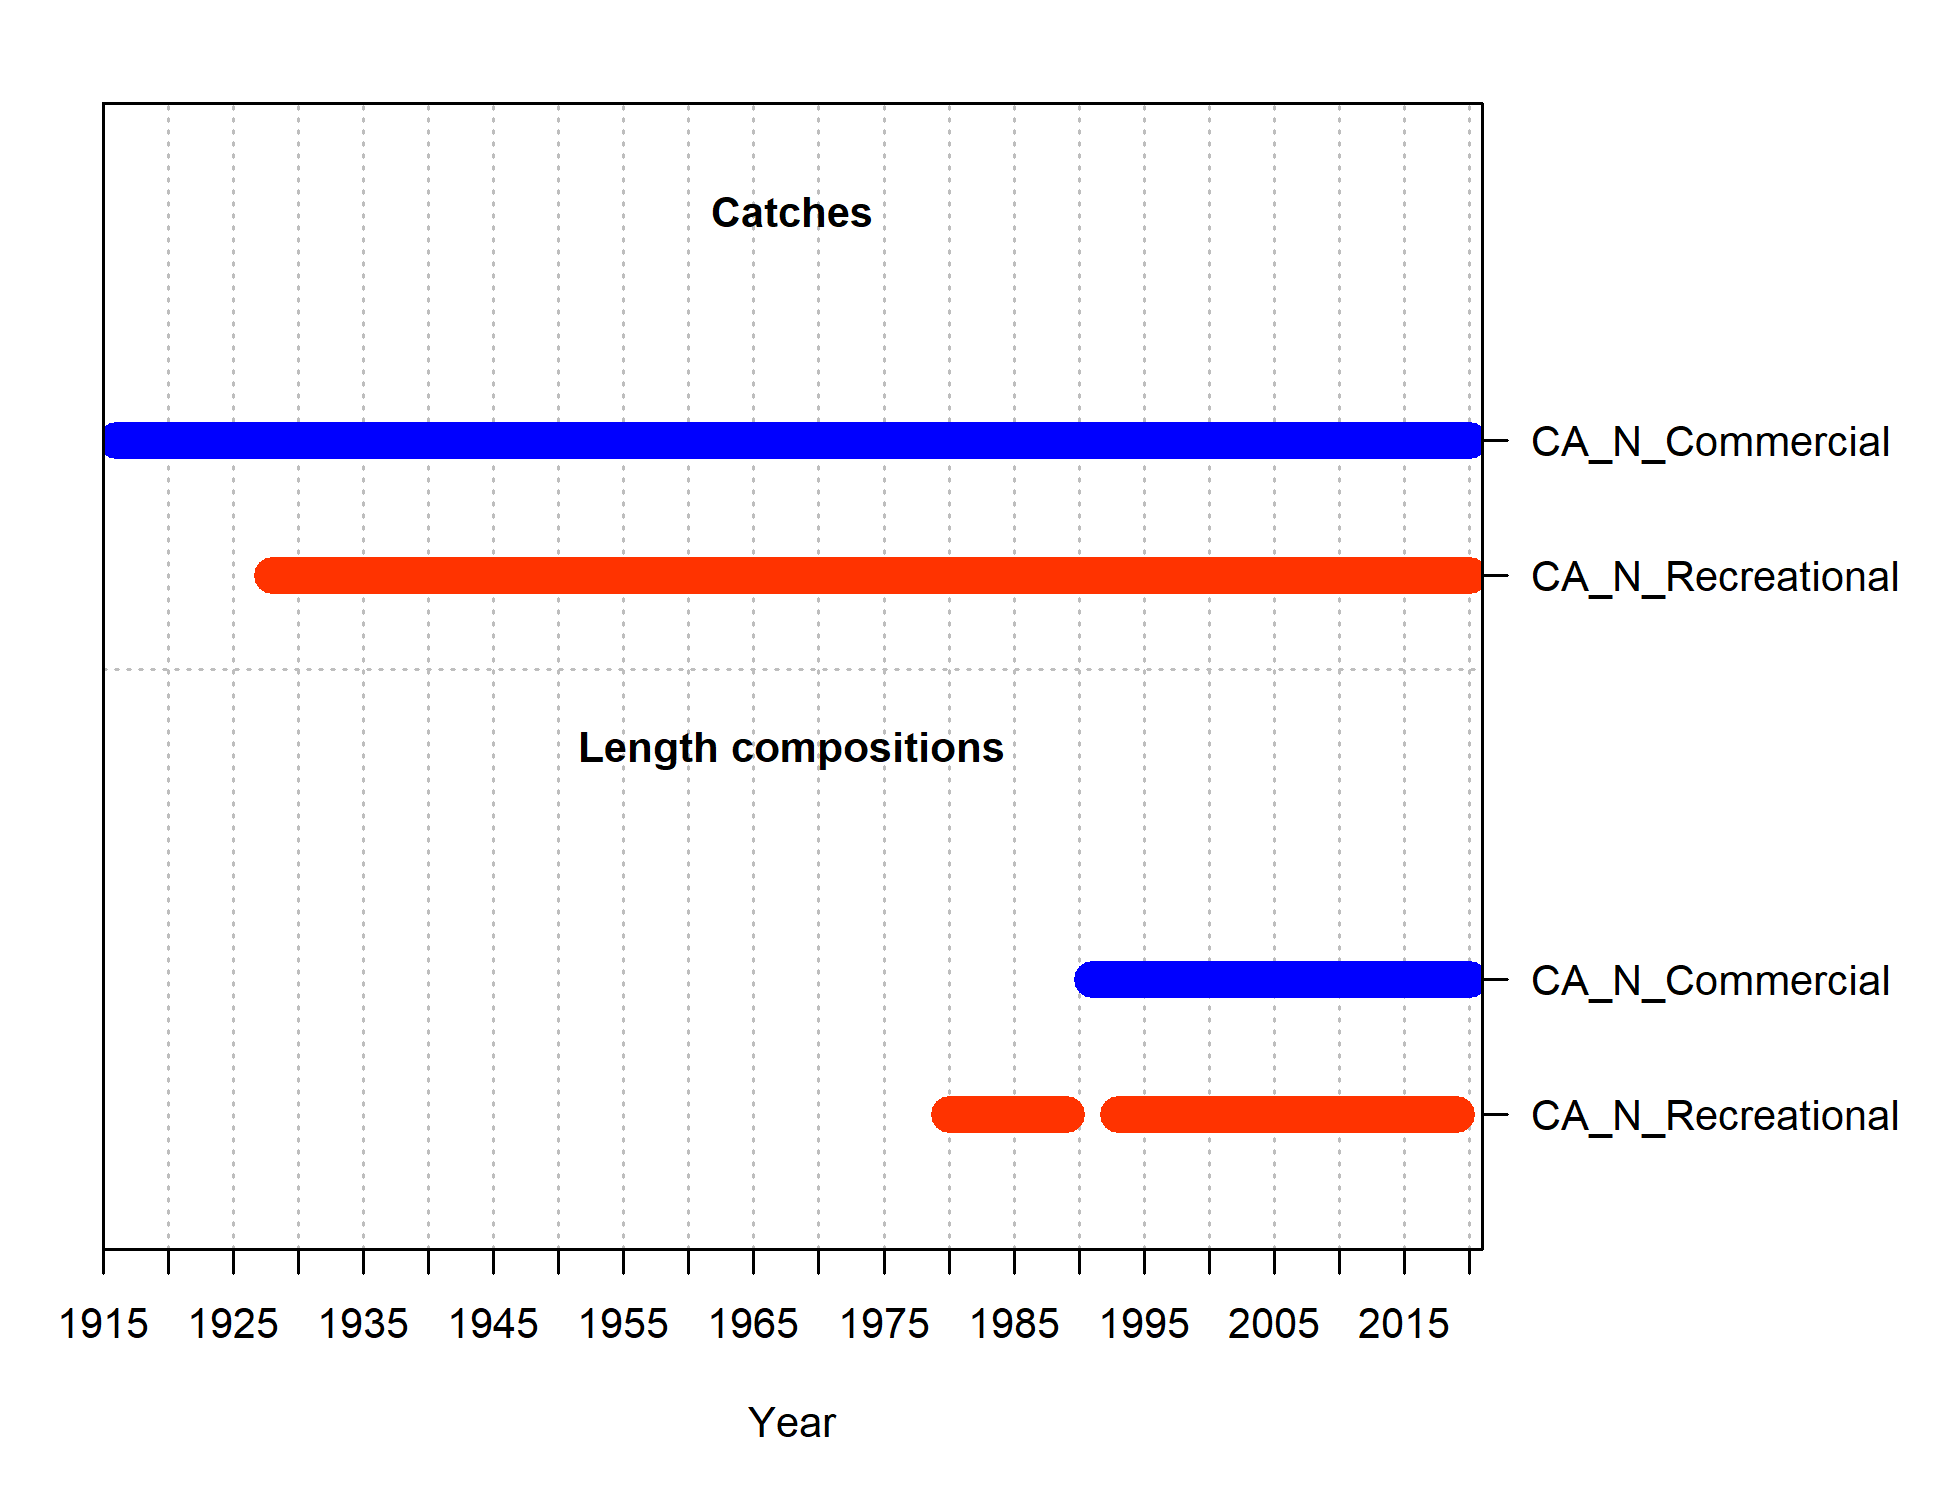
\includegraphics[width=1\textwidth,height=1\textheight]{C:/Assessments/2021/copper_rockfish_2021/models/wa/0.0_init_model/plots/data_plot.png}
\caption{Summary of data sources used in the base model.\label{fig:data-plot}}
\end{figure}

\tagmcend\tagstructend

\tagstructbegin{tag=Figure,alttext={Length at age in the beginning of the year in the ending year of the model.}}\tagmcbegin{tag=Figure}

\begin{figure}
\centering
\includegraphics[width=1\textwidth,height=1\textheight]{C:/Assessments/2021/copper_rockfish_2021/models/wa/0.0_init_model/plots/bio1_sizeatage.png}
\caption{Length at age in the beginning of the year in the ending year of the model.\label{fig:len-at-age}}
\end{figure}

\tagmcend\tagstructend

\tagstructbegin{tag=Figure,alttext={Weight at length by sex.}}\tagmcbegin{tag=Figure}

\begin{figure}
\centering
\includegraphics[width=1\textwidth,height=1\textheight]{C:/Assessments/2021/copper_rockfish_2021/models/wa/0.0_init_model/plots/bio5_weightatsize.png}
\caption{Weight at length by sex.\label{fig:weight}}
\end{figure}

\tagmcend\tagstructend

\tagstructbegin{tag=Figure,alttext={Maturity at length.}}\tagmcbegin{tag=Figure}

\begin{figure}
\centering
\includegraphics[width=1\textwidth,height=1\textheight]{C:/Assessments/2021/copper_rockfish_2021/models/wa/0.0_init_model/plots/bio6_maturity.png}
\caption{Maturity at length.\label{fig:maturity}}
\end{figure}

\tagmcend\tagstructend

\tagstructbegin{tag=Figure,alttext={Fecundity at a function of length.}}\tagmcbegin{tag=Figure}

\begin{figure}
\centering
\includegraphics[width=1\textwidth,height=1\textheight]{C:/Assessments/2021/copper_rockfish_2021/models/wa/0.0_init_model/plots/bio9_fecundity_len.png}
\caption{Fecundity at a function of length.\label{fig:fecundity}}
\end{figure}

\tagmcend\tagstructend

\tagstructbegin{tag=Figure,alttext={Selectivity at length by fleet.}}\tagmcbegin{tag=Figure}

\begin{figure}
\centering
\includegraphics[width=1\textwidth,height=1\textheight]{C:/Assessments/2021/copper_rockfish_2021/models/wa/0.0_init_model/plots/sel01_multiple_fleets_length1.png}
\caption{Selectivity at length by fleet.\label{fig:selex}}
\end{figure}

\tagmcend\tagstructend

\tagstructbegin{tag=Figure,alttext={Test figure.}}\tagmcbegin{tag=Figure}

\includegraphics[width=1\textwidth,height=1\textheight]{C:/Assessments/2021/copper_rockfish_2021/models/wa/0.0_init_model/plots/ts7_Spawning_output.png}

\tagmcend\tagstructend

\clearpage

\tagstructbegin{tag=H1}\tagmcbegin{tag=H1}

\hypertarget{references}{%
\section{References}\label{references}}

\leavevmode\tagmcend\tagstructend

\hypertarget{refs}{}
\begin{cslreferences}
\leavevmode\hypertarget{ref-dick_meta-analysis_2017}{}%
Dick, E. J., Sabrina Beyer, Marc Mangel, and Stephen Ralston. 2017. ``A Meta-Analysis of Fecundity in Rockfishes (Genus \emph{Sebastes}).'' \emph{Fisheries Research} 187 (March): 73--85. \url{https://doi.org/10.1016/j.fishres.2016.11.009}.

\leavevmode\hypertarget{ref-hamel_method_2015}{}%
Hamel, Owen S. 2015. ``A Method for Calculating a Meta-Analytical Prior for the Natural Mortality Rate Using Multiple Life History Correlates.'' \emph{ICES Journal of Marine Science: Journal Du Conseil} 72 (1): 62--69. \url{https://doi.org/10.1093/icesjms/fsu131}.

\leavevmode\hypertarget{ref-love_milton_probably_1996}{}%
Love, Milton. 1996. \emph{Probably More Than You Want to Know About the Fishes of the Pacific Coast}. Santa Barbara, California: Really Big Press.

\leavevmode\hypertarget{ref-ralston_documentation_2010}{}%
Ralston, Stephen, Don E. Pearson, John C. Field, and Meisha Key. 2010. ``Documentation of the California Catch Reconstruction Project.'' US Department of Commerce, National Oceanic; Atmospheric Adminstration, National Marine.

\leavevmode\hypertarget{ref-then_evaluating_2015-1}{}%
Then, A. Y., J. M. Hoenig, N. G. Hall, and D. A. Hewitt. 2015. ``Evaluating the Predictive Performance of Empirical Estimators of Natural Mortality Rate Using Information on over 200 Fish Species.'' \emph{ICES Journal of Marine Science} 72 (1): 82--92. \url{https://doi.org/10.1093/icesjms/fsu136}.
\end{cslreferences}
\end{document}
